% Supplementary material for the Marfa lights model paper (American Journal of Physics).
% Build:  latexmk -pdf marfa_ajp_SI.tex      (figures are read from ../figures/)
% Anonymous copy for review: latexmk -pdf -jobname=marfa_ajp_SI_anon -pdflatex='pdflatex %O "\def\anonbuild{1}\input{%S}"' marfa_ajp_SI.tex
\documentclass[11pt]{article}
\usepackage[margin=2.3cm]{geometry}
\usepackage{amsmath,amssymb}
\usepackage{graphicx}
\usepackage{booktabs}
\usepackage{tabularx}
\usepackage[section]{placeins}
\usepackage{url}
\usepackage{xurl}
\usepackage[hidelinks]{hyperref}
\graphicspath{{../figures/}}
\renewcommand{\thefigure}{S\arabic{figure}}
\renewcommand{\thetable}{S\arabic{table}}
\renewcommand{\theequation}{S\arabic{equation}}
\renewcommand{\thesection}{S\arabic{section}}
\setlength{\parskip}{0.4em}
\setlength{\parindent}{0pt}

\newif\ifanonymous
\anonymousfalse
\ifdefined\anonbuild\anonymoustrue\fi
\newcommand{\repo}{\ifanonymous[repository withheld for review]\else\url{https://github.com/zacharyslate/marfa-lights-investigation}\fi}
\newcommand{\website}{\ifanonymous[website withheld for review; a copy is included in this supplementary material as \texttt{website.zip}]\else\url{https://zacharyslate.github.io/marfa-lights-investigation/}\fi}
\newcommand{\kc}{k_{\mathrm{crit}}}

\title{Supplementary material for\\ ``Separating the known from the unknown at Marfa, Texas: line of sight, refraction, and photometry of the ordinary lights seen from the Marfa lights viewing area''}
\ifanonymous\author{[Author withheld for review]}\else\author{Zach Warren\\ \small Instituto de Cer\'amica y Vidrio (ICV), Consejo Superior de Investigaciones Cient\'{\i}ficas (CSIC), Madrid, Spain}\fi
\date{}

\begin{document}
\maketitle

This supplement gives the full methods behind the main paper, additional figures and tables, and a guide to the companion website. Equation, figure, table, and section numbers without an ``S'' refer to the main paper. All numbers are produced by the code in the project repository (\repo); the file that holds each result is named in the text.

\tableofcontents
\clearpage

%=======================================================================
\section{Data and provenance}\label{s:data}
%=======================================================================

The terrain and geoid files are pinned in \texttt{data/dem/MANIFEST.json} with their source URLs, sizes, SHA-256 checksums, and the servers' last-modified dates; the point-cloud tiles used are listed in \texttt{data/dem/ept\_nodes.json}, and the other inputs are stored in \texttt{data/inputs/}. Table~\ref{t:data} lists them.

\begin{table}[htbp]
\caption{Input data.}
\label{t:data}
\small
\begin{tabularx}{\textwidth}{p{3.6cm}Xp{3.6cm}}
\toprule
Layer & Product & Use \\
\midrule
Terrain, primary & USGS 3D Elevation Program 1-m DEM, lidar project TX\_WestTexas\_2018\_D19; 27 tiles of $10\times10$~km; quality level 2; Optech Galaxy sensor; collected February--May 2019 & every terrain sample inside the tiles \\
Terrain, fallback & USGS 1/3 and 1 arc-second DEMs (editions of 30 August 2022); 4 and 14 tiles & outside the lidar; skyline to 120~km \\
Lidar accuracy & project check-point test: non-vegetated RMSE$_z$ 5.6~cm (565 points), vegetated 95th percentile 21.6~cm (461 points) & terrain error model \\
Point cloud & the same lidar as Entwine Point Tiles (work units B3 and B7); 894 octree nodes, 29.4 million points around the grazing corridors & obstructions \\
Geoid & NOAA GEOID12B (the model used to produce the lidar heights); GEOID18 for sensitivity & NAVD88 $\to$ ellipsoidal heights \\
Roads & TxDOT Roadways, extract of 1 September 2026; 821 public-road features & lamp positions \\
Traffic & TxDOT annual average daily traffic (AADT), 2025 and two previous years & occupancy and rates \\
Railroads & USDOT/BTS North American Rail Network lines; FRA highway--rail crossing inventory (night-time through trains) & locomotive positions and rates \\
Towers & FCC Antenna Structure Registration, with registered lighting & fixed lights \\
Headlamps & UMTRI market-weighted beam patterns: low beam UMTRI-2004-23 Table 4; high beam UMTRI-2001-19 Table 6 & intensity \\
Signal lamps & FMVSS No.~108 photometric requirements as tabulated in NHTSA TP-108-13 & intensity brackets \\
Air clarity & National Park Service, Big Bend standard visual range & extinction \\
\bottomrule
\end{tabularx}
\end{table}

\textit{Observer.} The eye is 1.6~m above the viewing platform at $30.2751108^\circ$N, $103.8827973^\circ$W. The lidar resolves the platform as a pad 1.3--1.5~m above the surrounding ground, with its surface at 1494.80~m NAVD88; the 1 arc-second DEM, which does not resolve it, gives 1493.57~m. The geoid undulation there is $-21.19$~m.

\textit{Road centerline.} A hand-traced US-67 line used in an earlier version differs from the TxDOT centerline by 2.0~m (median), 4.9~m (90th percentile), and 9.3~m (maximum).

%=======================================================================
\section{Line-of-sight geometry}\label{s:geometry}
%=======================================================================

\subsection{Coordinates}

Each point is converted from geodetic longitude, latitude, and ellipsoidal height $h=H+N$ (orthometric height plus geoid undulation) to Earth-centered, Earth-fixed Cartesian coordinates on the WGS84 ellipsoid. Horizontal paths are geodesics, computed with Karney's algorithm\cite{Karney2013} (the \texttt{pyproj} implementation). The terrain between the eye $O$ and the lamp $T$ is sampled along the geodesic.

\subsection{Chord frame and the critical coefficient}

Let $\hat{\mathbf u}$ be the unit vector from the eye $O$ to the lamp $Q$ and $\hat{\mathbf w}$ the unit vector perpendicular to it in the plane spanned by $\hat{\mathbf u}$ and the mean ellipsoid normal. For each terrain sample $P_i$,
\begin{equation}
s_i=(\mathbf P_i-\mathbf O)\cdot\hat{\mathbf u},\qquad y_i=(\mathbf P_i-\mathbf O)\cdot\hat{\mathbf w}.
\end{equation}
With a constant refraction coefficient the ray is an arc lying above the chord by $\sigma_i(k)=ks_i(D-s_i)/2R$ (Eq.~2 and Appendix~A), where $R$ is the radius of curvature of the normal section of the ellipsoid in the azimuth $\alpha$ of the sight line, from Euler's formula,
\begin{equation}
\frac1R=\frac{\cos^2\alpha}{R_M}+\frac{\sin^2\alpha}{R_N},
\end{equation}
with $R_M$ and $R_N$ the meridional and prime-vertical radii of curvature at the mean latitude. The lamp is visible if and only if $k\ge\kc=\max_i 2Ry_i/[s_i(D-s_i)]$ (Eq.~3). The clearance at $k$ is $c(k)=\min_i[\sigma_i(k)-y_i]$, and the apparent elevation of the lamp at the eye is the chord elevation plus $kD/2R$.

\subsection{Sampling and end exclusions}

Samples are 2~m apart within 3~km of either end and 5~m apart in between. The first 5~m at the eye (the observer's own feet) and the last 3~m at the lamp (the car's body) are skipped. Table~\ref{t:conv} shows that the results have converged.

\begin{table}[htbp]
\caption{Convergence tests on US-67 (3095 points every 30~m from the US-90 junction in Marfa toward Presidio; lidar; 0.66~m lamp; $k=0.13$).}
\label{t:conv}
\small
\begin{tabular}{lc}
\toprule
Setting & Road in view (km) \\
\midrule
Reference: 2/5~m steps, 3~m exclusion at the lamp & 10.44\\
1/2~m steps & identical point by point (3095/3095)\\
30~m exclusion at the lamp & 10.47\\
60~m exclusion & 10.59\\
120~m exclusion (discards real terrain) & 11.19\\
\bottomrule
\end{tabular}
\end{table}

%=======================================================================
\section{How robust is ``visible''?}\label{s:robust}
%=======================================================================

\subsection{Margins}

The lamp margin $d_L$ is the change in lamp height that puts the ray exactly on the terrain, and $d_E$ is the same for the eye. Both follow from the clearance geometry; unit tests move the lamp or the eye by exactly the margin and check that visibility flips. No visible point on US-67 has $|d_L|>0.84$~m.

\subsection{Terrain-error Monte Carlo}

Each elevation source gets its own, independent error field along the sight line. For a source with correlation length $\ell$ we generate a unit-variance first-order autoregressive sequence on a uniform grid of spacing $\Delta=\min(\ell/4,5~\mathrm m)$,
\begin{equation}
\delta_{j+1}=\phi\,\delta_j+\sqrt{1-\phi^2}\,\xi_j,\qquad \phi=e^{-\Delta/\ell},
\end{equation}
with independent standard normal $\xi_j$, which has correlation $e^{-|\Delta s|/\ell}$. It is interpolated linearly to the terrain samples, rescaled to unit variance (midway between grid nodes linear interpolation lowers the variance to $(1+\phi)/2$, at worst 0.89, i.e.\ the standard deviation by 6\%), and multiplied by the standard deviation $\sigma$ of the source that supplied each sample. An independent eye-height error $\delta_{\mathrm{eye}}$ ($\sigma=0.15$~m) tilts the chord, adding $\delta_{\mathrm{eye}}(D-s)/D$. In each of 200 realizations the lamp is visible if the perturbed terrain stays below the ray; $P_{\mathrm{vis}}$ is the fraction of realizations in which it does. Only samples that could reach the ray within $6\sigma$ are evaluated.

The error statistics of the 1/3 and 1 arc-second models were measured against the lidar at 39\,807 points (\texttt{data/derived/los2/dem\_error.json}): standard deviations 0.56~m and 2.05~m (biases $-0.02$~m and $-0.09$~m). Semivariograms of the difference along random transects, fitted with the exponential model $\gamma(r)=\sigma^2(1-e^{-r/\ell})$ at lag $r$, with the sill fixed at $\sigma^2$ (the semivariogram of a field with correlation $e^{-r/\ell}$), give correlation lengths $\ell=70$~m and 125~m. For the lidar we use the reported non-vegetated RMSE, 0.056~m, and an assumed correlation length of 20~m.

\textit{Classes.} Visible: $P_{\mathrm{vis}}\ge0.95$ and still visible when 0.25~m of unresolved grass is added to the terrain. Hidden: $P_{\mathrm{vis}}\le0.05$. Marginal: otherwise. Between Shafter and Marfa (64.5~km) this gives 9.5~km visible, 0.5~km marginal, and 54.5~km hidden. The earlier implementation, which classed as ``visible'' any point with more than 5~m of clearance far from the car, gave 9.3, 7.4, and 47.9~km; almost all of its marginal road was an artifact of coarse terrain near the car.

\subsection{Obstructions from the point cloud}

On the 1-m grid of the DEM, a cell is marked obstructed (``dense'' rule) when it holds at least two returns and at least 25\% of its returns lie more than 0.3~m above the DEM surface; its height is raised to that of its highest return. Returns classed as noise (ASPRS classes 7 and 18) are ignored. An upper-bound variant (``max'') raises every cell to its highest return. As a check, 2.8 million ground returns differ from the DEM by a median of $-0.8$~mm (robust standard deviation 2.0~cm; 5th--95th percentile $-4.1$ to $+4.4$~cm). Only 0.8\% of corridor cells carry dense cover above 0.3~m.

\subsection{Results}

\begin{table}[htbp]
\caption{Road in view on US-67 (km; lidar with obstructions; Marfa to Presidio) versus lamp height and refraction coefficient.}
\label{t:lampk}
\small
\begin{tabular}{lccccc}
\toprule
Lamp height & $k=0$ & 0.13 & 0.25 & 0.5 & 1 \\
\midrule
0.56~m & 9.45 & 9.72 & 9.96 & 11.07 & 11.49\\
0.66~m (reference headlamp) & 9.69 & 9.93 & 10.14 & 11.22 & 11.61\\
0.86~m (tail lamps) & 9.90 & 10.14 & 10.32 & 11.52 & 11.88\\
1.12~m (high-mounted stop lamp) & 10.35 & 10.59 & 10.71 & 11.76 & 12.15\\
1.37~m & 10.59 & 10.83 & 10.98 & 12.09 & 12.42\\
2.5~m & 11.70 & 11.94 & 12.24 & 13.14 & 13.47\\
4.0~m (truck clearance lamps) & 13.50 & 13.77 & 14.64 & 14.97 & 15.33\\
\bottomrule
\end{tabular}
\end{table}

The ``max'' obstruction variant gives 9.84~km at the reference settings, and uniform clutter of 0.25, 0.5, and 1~m added to all terrain more than 10~m from both ends gives 9.36, 8.67, and 2.04~km (the 1-m case is an unrealistic bound). The limiting terrain sample lies a median 3.0~km from the car, and within 100~m of it for only 9\% of points. Figure~\ref{f:sections} shows cross-sections along four bearings.

\begin{figure}[htbp]
\centering
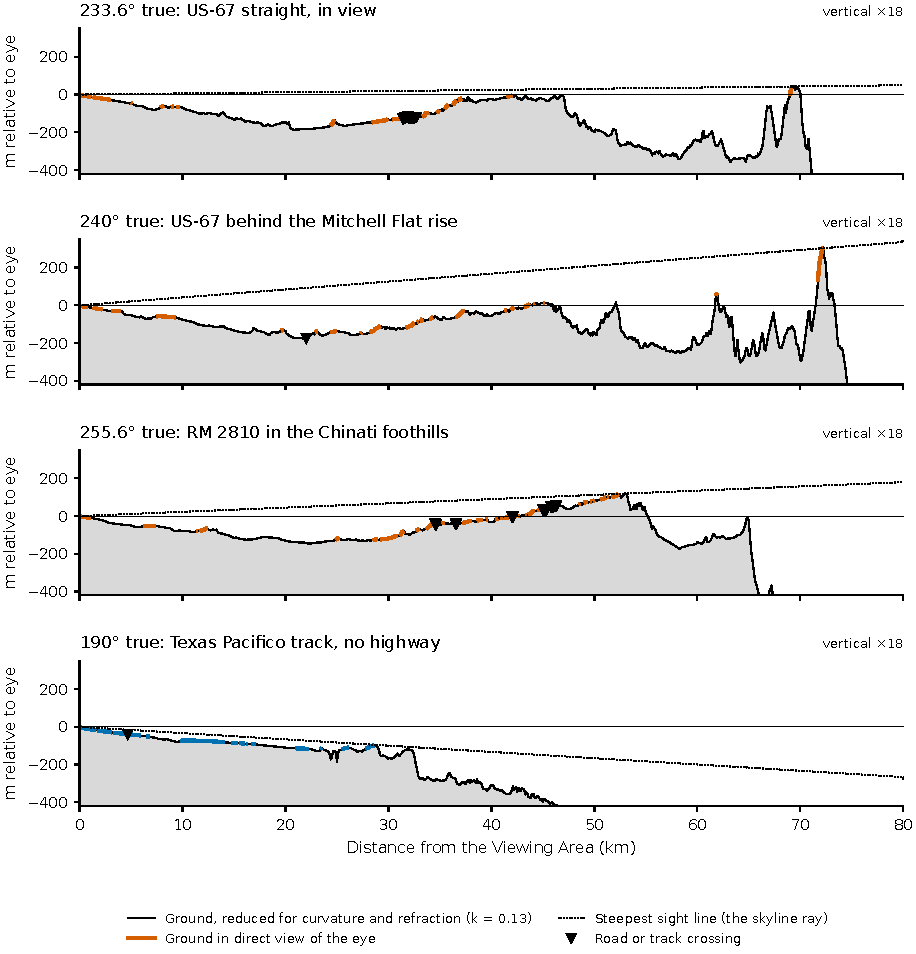
\includegraphics[width=0.85\textwidth]{fig04_sightlines.pdf}
\caption{Terrain cross-sections from the platform, reduced for curvature and refraction ($k=0.13$), exaggerated $18\times$ vertically, along (a) $233.6^\circ$ true, where the view skims the far slope that carries a straight stretch of US-67 in view; (b) $240^\circ$, where a low rise on Mitchell Flat hides the highway; (c) $255.6^\circ$, across RM~2810 in the Chinati foothills; (d) $190^\circ$, along the Texas Pacifico railroad, with no highway. Colored: ground in direct view of the eye. Triangles: road or track crossings.}
\label{f:sections}
\end{figure}

%=======================================================================
\section{Refraction}\label{s:refraction}
%=======================================================================

\subsection{Local refraction coefficient}

A ray at elevation $e$ in a horizontally stratified atmosphere curves toward the denser air with curvature $\kappa=-(1/n)(dn/dz)\cos e$. With $n-1=cP/T$ ($c=79.0\times10^{-6}$~K/hPa at visible wavelengths) and hydrostatic pressure, $dP/dz=-g_0P/(R_dT)$ ($g_0$ the acceleration of gravity, $R_d$ the gas constant of dry air), one finds, for $n\approx1$ and $\cos e\approx1$,
\begin{equation}
k=R\kappa \approx R\,c\,\frac{P}{T^2}\left(\frac{g_0}{R_d}+\frac{dT}{dz}\right)\approx503\,\frac{P}{T^2}\left(0.0343+\frac{dT}{dz}\right),
\end{equation}
Eq.~(4) of the main paper.\cite{Hirt2010} Here $Rc=503$~m\,K/hPa for $R=6371$~km, and $g_0/R_d=0.0342$~K/m is the autoconvective lapse rate, which Hirt \textit{et al.}\ give as 0.0343; the difference changes $k$ by less than 0.001. At 850~hPa and 283~K the prefactor $503P/T^2$ is 5.34~m/K. (The code computes the same relation from $c$, $g_0$, and $R_d$; a unit test checks it against a numerical derivative of $n(z)$ in a hydrostatic atmosphere.)

\subsection{Ray tracing}

In the chord frame the ray obeys $y''=-k(a)/R$, where $a=y-y_{\mathrm{ground}}(s)$ is the height above the local ground (Eq.~5); for the elevation angles here ($<1^\circ$) the paraxial error is of relative order $10^{-4}$. We launch a fan of rays from the eye, integrate each to $s=D$, discard rays that meet the terrain outside the end exclusions, and find the roots of $y(D;\theta)=0$ by linear interpolation between neighboring rays. Each root is an image with apparent elevation equal to the chord elevation plus $\theta$; no root means the lamp is hidden, and more than one root is a mirage.

\textit{Profiles.} Temperature follows the terrain. The stable boundary layer has the exponential form\cite{Stull1988} $T(a)=T_0+\Delta T(1-e^{-a/h})+\gamma a$, so $dT/dz=(\Delta T/h)e^{-a/h}+\gamma$. Weak: $\Delta T=3$~K, $h=50$~m (surface gradient 0.06~K/m); moderate: 6~K, 30~m (0.2~K/m); strong: 10~K, 20~m (0.5~K/m). Also: neutral ($-0.0098$~K/m), isothermal, and an elevated inversion of 4~K between 40 and 60~m above a mixed layer. These are brackets, not a climatology; Hirt \textit{et al.} measured gradients of 1--2~K/m at 1.8~m above grass shortly after sunset, stronger than any here, but the rays of interest are within 2~m of the ground only near their two ends.

\textit{Bound.} If $k\le k_{\max}$ everywhere, then $y''\ge-k_{\max}/R$ with fixed end points, so every ray lies below the constant-$k_{\max}$ arc, and a lamp with $\kc>k_{\max}$ is hidden. With $k_{\max}=2.82$ in our profiles, points with $\kc>2.9$ need no tracing; 212 of 1548 points (Marfa to Presidio, every 60~m) remain.

\textit{Tests.} A constant gradient reproduces the constant-$k$ arc and horizon; the reach of a surface duct matches its analytic value.

\begin{table}[htbp]
\caption{Ray tracing results (US-67, 0.66~m lamp, 60-m spacing; \texttt{data/derived/los2/trace\_us67.json}). $k_{\mathrm{eq}}$: median constant $k$ reproducing the traced arrival angle. Lift: rise in apparent elevation relative to $k=0.13$. The neutral case differs from Table~I of the main paper through the coarser sampling.}
\label{t:trace}
\small
\begin{tabular}{lccc}
\toprule
Profile & In view (km) & $k_{\mathrm{eq}}$ & Lift, median / max (arcmin)\\
\midrule
Neutral & 9.78 & 0.13 & 0 / 0\\
Isothermal & 9.90 & 0.18 & 0.4 / 0.6\\
Weak stable layer & 10.86 & 0.30 & 1.4 / 1.7\\
Moderate stable layer & 10.92 & 0.47 & 2.9 / 4.3\\
Strong stable layer & 11.28 & 0.67 & 4.5 / 7.5\\
Elevated inversion, 40--60~m & 9.66 & 0.36 & 1.8 / 2.8\\
\bottomrule
\end{tabular}
\end{table}

\textit{Multiple images.} The elevated inversion gives three to five images at five road points (60-m samples between 18.6 and 24.4~km from Marfa), 1--8 arcseconds apart. They persist when the step falls from 5 to 1~m and the fan density rises sevenfold, but they cannot be resolved by the eye.

\begin{figure}[htbp]
\centering
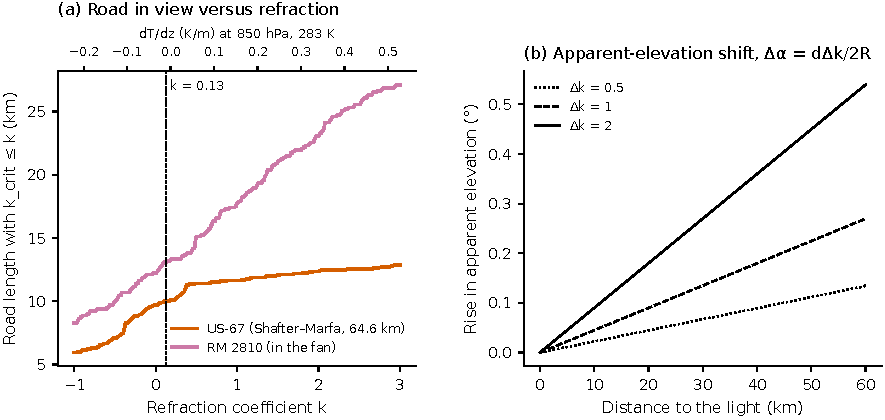
\includegraphics[width=0.85\textwidth]{fig05_refraction.pdf}
\caption{(a) Road in view versus refraction coefficient (constant-$k$ model; US-67 between Shafter and Marfa, and RM~2810 within the viewing fan); the top axis gives the equivalent temperature gradient at 850~hPa and 283~K from Eq.~(4). (b) Rise in apparent elevation of a light at distance $d$ for a change $\Delta k$, $\Delta\alpha=d\,\Delta k/2R$.}
\label{f:refraction}
\end{figure}

%=======================================================================
\section{Photometry}\label{s:photometry}
%=======================================================================

\subsection{Heading, grade, and view angles}

The heading $\psi$ at each 60-m road sample is the geodesic azimuth between its two neighbors along the TxDOT centerline. The grade $g$ is the lidar height difference between points 25~m ahead and 25~m behind along $\psi$, divided by 50~m, and clipped to $\pm8\%$ (no point on US-67 between Shafter and Marfa needed clipping). Both directions of travel are evaluated. The angles of the observer in the lamp frame are $h=\beta-\psi$, wrapped to $(-180^\circ,180^\circ]$, and $v=\epsilon_Q-\arctan g-\delta_{\mathrm{aim}}$, with $\epsilon_Q=-e_O-D/R+kD/2R$ (Eq.~6). The term $-e_O-D/R$ is the elevation of the chord at the lamp: the verticals at the eye and the lamp differ by the central angle, which $D/R$ reproduces to better than $1''$ at these ranges. Refraction raises the ray at both ends by $kD/2R$. For equal heights and no refraction both ends see the chord at $-D/2R$. Unit tests check the formula against exact three-dimensional geometry.

On US-67 the platform lies $3^\circ$--$33^\circ$ to the right of northbound drivers (5th--95th percentile; median $14^\circ$) and $0.6^\circ$ below to $2.5^\circ$ above their lamp axis (median $+0.8^\circ$). Southbound drivers have it $3^\circ$--$33^\circ$ off their rear axis.

\subsection{Headlamp tables}

The UMTRI tables\cite{Schoettle2004,Schoettle2001} give the 25th, 50th, and 75th percentiles of single-lamp luminous intensity at 12.8~V on a grid of 45 horizontal angles ($45^\circ$L to $45^\circ$R) and 25 vertical angles ($5^\circ$D to $7^\circ$U). The low-beam sample is the 20 best-selling U.S. vehicles of model year 2004 (39\% of sales); the high-beam sample is the sales-weighted U.S. fleet of about 2000. The tables were read from the text layer of the published PDF reports and assigned to columns by position; every one of the 1125 cells of each table satisfies $p_{25}\le p_{50}\le p_{75}$, and the values at $H$-$V$ (low beam 5758/8830/11\,846~cd; high beam median 37\,005~cd) were checked against the printed tables. Intensities are interpolated linearly in $\log_{10}I$ (floor 0.5~cd). Beyond $|h|=45^\circ$ the intensity is either held at its $45^\circ$ value or set to the regulatory minimum of the front position and side-marker lamps; the difference matters for no US-67 point in view. Two lamps are summed, and nothing is emitted forward for $|h|>90^\circ$.

\subsection{Signal lamps}

Table~\ref{t:fmvss} lists the FMVSS No.~108 values used.\cite{TP108} The minimum is interpolated linearly in $\log I$ between the tabulated angles, held at the last tabulated value out to $45^\circ$ (the angle to which the lamps must be visible), and set to zero beyond; the maximum is applied out to $45^\circ$.

\begin{table}[htbp]
\caption{FMVSS No.~108 photometry used for signal lamps (one lighted section; candela; horizontal angles off the lamp axis), as tabulated in NHTSA TP-108-13.}
\label{t:fmvss}
\small
\begin{tabular}{lccccc}
\toprule
Lamp & Min., $0^\circ$--$5^\circ$ & Min., $10^\circ$ & Min., $20^\circ$ & Max. & Number per car\\
\midrule
Tail lamp & 2.0 & 0.8 & 0.3 & 18 & 2\\
Stop lamp & 80 & 40 & 10 & 300 & 2\\
High-mounted stop lamp & 25 & 16 & -- & 160 & 1\\
\bottomrule
\end{tabular}
\end{table}

\subsection{Transmission, magnitude, and threshold}

The meteorological optical range is $V=\ln20/b$ for an extinction coefficient $b$; the NPS standard visual range\cite{NPS_BIBE} is $3.912/b$, so $V=0.766\times$ the visual range. The reported 55, 90, and 165~miles become 68, 111, and 203~km. The magnitude scale of Eq.~(8) follows from Schaefer's relation\cite{Schaefer1993} between point-source illuminance and magnitude: $m=0$ corresponds to $E=2.5\times10^{-6}$~lx. The Crumey threshold (Eq.~9) is his fit\cite{Crumey2014} for $20<\mu<22$~mag\,arcsec$^{-2}$; the field factor $F$ collects the observer's acuity, experience, and conditions. Table~\ref{t:mlim} gives $m_{\mathrm{lim}}$ over the ranges used.

\begin{table}[htbp]
\caption{Naked-eye limiting magnitude from Eq.~(9).}
\label{t:mlim}
\small
\begin{tabular}{lcccc}
\toprule
$\mu$ (mag\,arcsec$^{-2}$) & $F=1.4$ & 2.0 & 2.4 & 4.0\\
\midrule
20.5 & 6.05 & 5.67 & 5.47 & 4.91\\
21.0 & 6.25 & 5.86 & 5.66 & 5.11\\
21.5 & 6.44 & 6.05 & 5.85 & 5.30\\
22.0 & 6.63 & 6.24 & 6.04 & 5.49\\
\bottomrule
\end{tabular}
\end{table}

\subsection{Further results}

Where a northbound car's headlamps are in view, the low-beam gradient $d\log_{10}I/dv$ at the observer's position is $-0.25$ per degree (median; interquartile $-0.14$ to $-0.37$), a factor of 1.4--2.3 per degree. Within one window longer than a single sample the brightness changes by a median 1.1 magnitudes (maximum 4.9); between successive 60-m samples (2~s at 30~m/s) by more than 0.8 magnitudes one time in ten (maximum 2.7). On RM~2810 only the direction toward Marfa faces the platform ($|h|$ from $3^\circ$ to $42^\circ$, median $18^\circ$): low-beam median $m=4.0$, brightest $-0.7$; high beam brightest $-2.4$.

%=======================================================================
\section{One car and occupancy}\label{s:occupancy}
%=======================================================================

A window is a maximal run of consecutive 60-m samples in view ($P_{\mathrm{vis}}\ge0.5$ for the lamp's height); its duration at speed $u$ is its length divided by $u$. Windows shorter than 60~m cannot be resolved. For vehicles arriving at random with one-way flow $q$, the number in a road section of length $L$ at speed $u$ is Poisson with mean $qL/u$ (Eq.~10), and the probability that at least one is in view is $1-e^{-qL/u}$. Each vehicle produces one appearance per window, so a flow $q$ produces $q$ times 18 appearances per hour on US-67.

For the occupancy we use the 2025 AADT (1121 and 1383 vehicles per day at stations 189D5 and 189H5A, both directions), a daily-mean one-way flow of 23--29 vehicles per hour. The rate map of Sec.~\ref{s:mask} uses, more conservatively, the highest of the three most recent annual counts (2331 and 1549). No hourly night-time count exists for this road; night flows are lower than the daily mean, and a traffic count during an observing session should replace these values.

%=======================================================================
\section{Known-source catalogue, mask, and rate map}\label{s:mask}
%=======================================================================

\subsection{Catalogue}

The catalogue contains: US-67 (60-m samples) and the state roads in the viewing fan (RM~2810, US-90, US-67/90 beside the platform, FM~170, SH~118, RM~169, FM~1112, SH~17; 120-m samples; lamp 0.66~m); the Union Pacific and Texas Pacifico railroads (locomotive headlight at 4~m); every FCC-registered tower with registered lighting (top light; 29 of 65 registered structures in the area are lit, and 7 of those show their top light at $k=0.13$); the towns of Marfa, Shafter, Presidio, and Ojinaga (direct light where in view for some $k\le1$, otherwise a skyglow band from the skyline to $0.5^\circ$ above it over $\pm1^\circ$ of bearing); and the tethered aerostat at $292.9^\circ$ (a full-height column, because its altitude varies).

\subsection{Known-source mask}

Each source $i$ with $\kc\le1$ occupies the vertical segment of apparent elevation from $\alpha_i(\max(\kc,0))$ to $\alpha_i(1)$, where $\alpha_i(k)=\alpha_i(0.13)+d_i(k-0.13)/2R$. Neighboring samples of the same road or track less than 1~km apart are joined. The union is widened by the observer's pointing error, $\pm0.3^\circ$ in bearing and $\pm0.1^\circ$ in elevation for photographic pointing (a skyline-referenced photograph or a theodolite) and $\pm3^\circ$ by $\pm0.25^\circ$ for compass pointing, rasterized at $0.02^\circ\times0.04$~mrad, and converted to polygons (\texttt{data/derived/zos.json}). Within the $120^\circ$ fan, in the band 5~mrad deep below the skyline, the mask covers 30\% at photographic and 73\% at compass pointing. Towns beyond the terrain model (Presidio and Ojinaga) are treated as skyglow.

\subsection{Rate map}

The expected number of catalogued transient lights per hour in each patch of the view is
\begin{equation}
\lambda=\sum_s q_s\,P_{\mathrm{det},s},
\end{equation}
where for a road $q_s=\mathrm{AADT}\times0.02/2$ per direction (2\% of daily traffic per night hour; no measured night share was found) and $P_{\mathrm{det}}=p_{\mathrm{high}}[m_{\mathrm{high}}\le m_{\mathrm{lim}}]+(1-p_{\mathrm{high}})[m_{\mathrm{low}}\le m_{\mathrm{lim}}]$ with $p_{\mathrm{high}}=0.25$ (high-beam use on isolated rural roads\cite{Reagan2017}), $m_{\mathrm{lim}}=5.86$, and $V=111$~km. For a railroad $q$ is the largest number of night-time through trains reported at any of its crossings divided by 12~h. A road contributes its rate once per patch; rates are the maximum along one line and the sum across lines. Permanent lights (towers, towns, the aerostat) are a separate ``fixed light'' layer.

In the band 5~mrad below the skyline, the fraction of the view with $\lambda<0.01$~h$^{-1}$ and no fixed light (``quiet'') is 0.789 on a standard night ($k=0.13$), 0.763 with strong refraction ($k=1$), and 0.782 if southbound tail lamps at the FMVSS maximum are counted. With compass pointing it is 0.374. Figure~\ref{f:rate} shows the map (\texttt{data/derived/weighted\_zone.json}).

\begin{figure}[htbp]
\centering
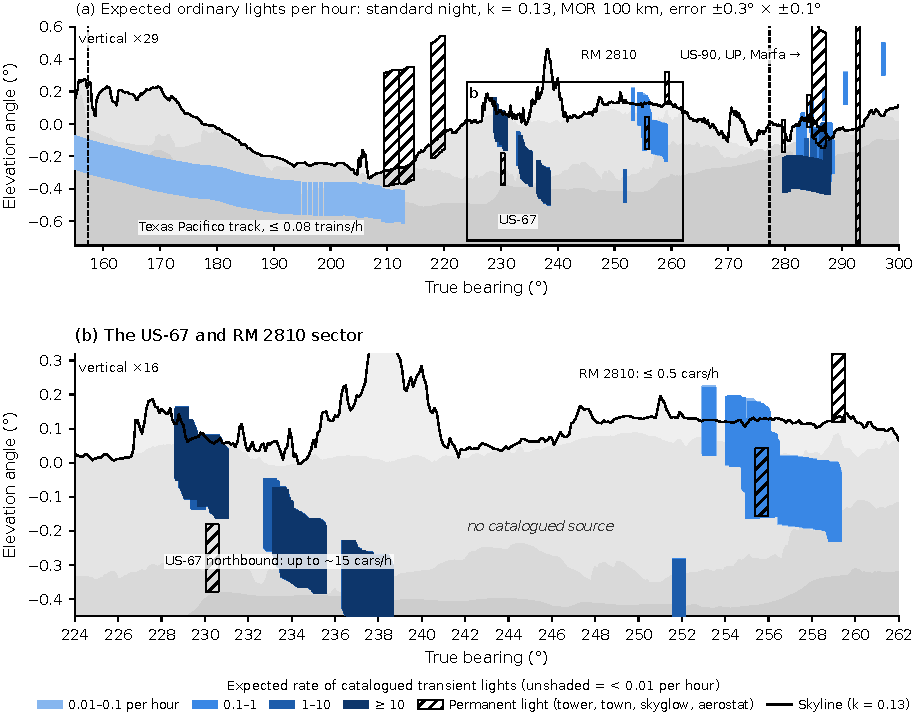
\includegraphics[width=0.9\textwidth]{fig06_weighted_zone.pdf}
\caption{Expected rate of catalogued transient lights (per hour) across the view on a standard night ($k=0.13$, $V=111$~km, pointing error $\pm0.3^\circ\times\pm0.1^\circ$), with fixed lights hatched. (a) $155^\circ$--$300^\circ$, vertical scale exaggerated $29\times$; the box is the region of (b). (b) The US-67 and RM~2810 sector, $224^\circ$--$262^\circ$, exaggerated $16\times$. Northbound US-67 traffic reaches about 23 lights per hour and RM~2810 at most 0.5; the Texas Pacifico track carries at most 0.08 trains per hour.}
\label{f:rate}
\end{figure}

%=======================================================================
\section{Photograph analysis}\label{s:photos}
%=======================================================================

\textit{Data.} Ten frames taken from the platform on 21 November 2018 with a Sony ILCE-6300 (APS-C, 23.5~mm sensor, 6000~px wide) and an E~55--210~mm lens at 210~mm (nominal scale 936~px per degree), exposures 1/25~s to 45~s. A sunset frame from the same camera calibrates its clock.

\textit{Registration.} In each frame the sky--land boundary is traced where red minus blue drops sharply. A rectilinear camera model with four parameters (azimuth $A_0$, elevation $E_0$, roll, focal-length scale) is fitted to the modeled skyline ($k=0.13$) by robust least squares. Residuals are 0.005--0.017$^\circ$. The fitted scale is 0.974--0.977 in every frame, an effective focal length near 205~mm. The best alternative pointing fits 1.4 to 10 times worse. Matching the solar disc in the sunset frame to its computed position (Astronomy Engine,\cite{AstroEngine} standard refraction) shows the camera clock 59~min fast, so the frames were taken at 18:12--18:26 CST, 20--35~min after sunset.

\textit{Detection.} A high-pass image (the frame minus its $21\times21$~px median) is thresholded at 7 robust standard deviations; detections must have 4--600~px and lie between the modeled 10-km ridge line and the skyline. A contrast rule (peak/median $\ge1.20$) was set after inspecting the detections; results are reported with and without it and do not change.

\textit{Independent sightings.} Frames seconds apart show the same vehicles, so the unit of analysis is a sighting within a burst (frames 04+05, 06+07, 08, 09, 10). Two detections in one burst are the same vehicle if they lie on the same road and their along-road separation is within what a vehicle at $\le45$~m/s covers between frames, plus 60~m. This gives eight sightings.

\textit{Statistic and null model.} The statistic is the median angular distance from the sightings to the modeled curve of visible road (piecewise linear between consecutive in-view 60-m samples). The null places the same number of random points per burst uniformly in each frame's ground band. The observed median is $0.0085^\circ$ (maximum $0.013^\circ$), against a null median of medians of $0.28^\circ$; only 1.4\% of the band lies within $0.0085^\circ$ of visible road. The exact probability that at least 4 of 8 random points fall that close (Poisson-binomial, with each burst's own fraction) is $3\times10^{-6}$; because a median of 8 values can only be as small as $x$ if at least four values are, this is an upper bound on the chance of a median as small as observed ($2\times10^{-6}$ without the contrast rule); no one of 4000 Monte Carlo draws was as close.

\textit{Visible--hidden boundary.} 48--50\% of the US-67 samples that project into each frame are modeled as hidden, yet the road sample nearest each of the eight sightings is a visible one. If the model's split had no predictive power, the probability would be the product of the frames' visible fractions, about 0.005.

\textit{Speeds.} Frames 04$\to$05 (6~s): $179\pm30$~m along the road, 30~m/s (17--48~m/s at $2\sigma$), including 1-s timestamp resolution and a $0.006^\circ$ position error. Frames 06$\to$07 (2~s): 41~m/s (16--114~m/s); a second pair is unconstrained because the road points almost at the platform there.

\textit{Long exposure.} In the 45-s frame, streaks are found without the model (7 robust standard deviations, below the skyline, width $\ge60$~px, aspect ratio $\ge5$). Streak 1 ($236.90^\circ$--$237.36^\circ$) lies a median $0.0049^\circ$ from visible road; streak 2 ($233.93^\circ$--$234.02^\circ$, 88~px) lies $0.028^\circ$ from it and is of undetermined origin.

\textit{Limitations.} Because the pointing is fitted to the modeled skyline, these tests measure internal consistency, not absolute pointing. The frames are not photometrically calibrated and do not constrain $k$, which is degenerate with $E_0$.

%=======================================================================
\section{Verification}\label{s:verify}
%=======================================================================

Forty-five unit tests (\texttt{analysis/tests/}) pass:
\begin{itemize}\itemsep0pt
\item \textit{Geometry:} Euler normal-section radius; smooth-Earth horizon distance for $k=0$, 0.13, 0.5; dip of a sea-level horizon; $\kc$ against brute force on random terrain; an isolated ridge against its analytic $\kc$; the multi-lamp engine against the single-lamp engine; lamp and eye margins flip visibility; fine sampling near both ends; missing terrain raises an error; clutter raises $\kc$.
\item \textit{Monte Carlo:} statistics of the correlated error field; the deterministic limit; the analytic probability for a pure eye-height error.
\item \textit{Ray tracer:} Eq.~(4) gives the standard value; constant gradients reproduce constant-$k$ arcs and horizons; the reach of a surface duct matches its analytic value.
\item \textit{Equations} (\texttt{test\_equations.py}, independent of the model code): the curvature drop and horizon against an exact sphere; the parabolic sag against the exact circular arc; $\kc$ as the visibility threshold; the refraction coefficient of Eq.~(4) against a numerical derivative of $n(z)$ in a hydrostatic atmosphere; the comparison bound for height-dependent $k$; the elevation at the lamp, Eq.~(6), against exact three-dimensional geometry; the pitch sign; optical and visual range; the magnitude constant (from Schaefer's foot-candle form, and the Sun as a check); the Crumey values; the occupancy, Eq.~(10), against a simulation of random traffic; the angular drift rate; Euler's radius; the autoregressive error field; and the conservativeness of the median test.
\item \textit{Photometry:} tabulated UMTRI values; the magnitude scale; the definition of optical range; the Crumey relation; sign conventions of $h$ and $v$; level-ground symmetry; signal-lamp brackets.
\end{itemize}

An earlier, independent implementation (1 arc-second terrain, 15-m step, 30/60-m end exclusions, spherical Earth) is reproduced when run with its settings: visibility agrees for 1075 of 1077 points, and its ``clearance'' equals our lamp margin to $-0.03$~m (median). Its azimuths were $0.117^\circ$ too large on average ($0.145^\circ$ at most) and its distances off by up to 72~m, from mixing spherical and ellipsoidal geometry. The photograph registration absorbed exactly this azimuth offset in the earlier analysis.

%=======================================================================
\section{The companion website}\label{s:website}
%=======================================================================

The model is published as a website, \website, built from the same derived data. It works on phones and offline once loaded. Its pages:
\begin{itemize}\itemsep0pt
\item \textit{Map and light identifier:} a map and panorama of the view with every catalogued source (the US-67 line of sight, refraction, railroads, airfields, towers, and towns). The observer enters the bearing and elevation of a light, uses the phone compass, or taps the map or panorama, and the tool lists every known source on that line within a chosen window and, for roads, how bright a car there would look.
\item \textit{Sky finder:} points the phone camera at the view and draws the skyline, US-67, RM~2810, towers, and stars on the live image; after calibration on a known light it records a calibrated bearing and elevation.
\item \textit{Report a sighting:} a form that checks a reported light against every known source and keeps the report on the user's device until the user chooses to send it.
\item \textit{Sight lines:} where US-67 can be seen from the platform, point by point.
\item \textit{Science:} the figures of this work with plain-language explanations.
\end{itemize}

\ifanonymous A copy of the website is included as \texttt{website.zip}; open \texttt{index.html} in a browser.\fi

%=======================================================================
\section{Reproducing the results}\label{s:reproduce}
%=======================================================================

From the repository root, with the Python environment described in the repository:
\begin{verbatim}
cd analysis
python -m marfa.fetch_dem --download       # terrain, point cloud, geoid
python -m marfa.fetch_dem --verify         # check against MANIFEST.json
python -m marfa.run_los us67  --dem lidar  # line of sight, US-67
python -m marfa.run_los roads --dem lidar --spacing 60
python -m marfa.run_trace                  # ray tracing
python -m marfa.run_photometry
python -m marfa.run_traffic
python -m marfa.export_site
cd ..
python analysis/headlight_model.py
python analysis/build_site_data.py
python analysis/zone_of_skepticism.py      # known-source mask
python analysis/weighted_zone.py           # rate map
python analysis/pub_figures.py
python analysis/photo_figures.py
python analysis/manuscript_figures.py
pytest analysis/tests
\end{verbatim}
The exact options of each step are given in \texttt{publication/README.md}.

\bibliographystyle{unsrt}
\bibliography{refs,refs_si}

\end{document}
